\section{Learning algorithm}  
\label{algorithm}
In this section, we consider three instances of Angluin's MAT framework.
In the first instance, the teacher knows an MMT $\M$, and the learner poses membership queries
to learn the untimed behaviors of $\M$, and equivalence queries to check whether an hypothesis is correct.
In the second instance, the teacher also knows an MMT $\M$, but now the 
learner performs timed experiments to learn about the
timed words of $\M$, and poses equivalence queries and lookahead queries.
The third instance is the well known setting (see e.g.\ \cite{Nie03,RSBM09}) 
in which the teacher knows an (untimed) Mealy machine $\A$,
and the learner performs membership and equivalence queries.
%
We will show how an untimed teacher for MMTs can be implemented using a timed teacher for MMTs,
and how an untimed learner for MMTs can be implemented using a Mealy machine learner.
%This will allow us to use existing algorithms for learning Mealy machines,
%as implemented for instance in LearnLib \cite{RSBM09}, as part of an algorithm to learn MMTs. 

\ifshort
Note that for an untimed behavior $\beta$, the set $\zone{\beta}$ of valuations that can be reached with a timed behavior $\sigma$ with $\untime(\sigma) = \beta$ can be symbolically represented using DBMs \cite{Di89}.
We can do this since the transition relations $\xrightarrow{d}$ and $\xrightarrow{i_1/o_1, \rho_1}$ can be decomposed 
into elementary operations on DBMs such as reset, conjunction, and delay successors \cite{BengtssonY03}.
This allows us to compute whether an untimed behavior $\beta$ is feasible ($\zone{\beta}$ is empty), and
whether a timer $x$ may expire after $\beta$ ($\zone{\beta}$ contains a valuation in which $x$ is minimal).
\fi

\subsection{An untimed MAT framework for learning MMTs}
Given the equivalence of the timed and the untimed semantics of MMTs, it is natural to also 
consider an untimed setting, in which a learner tries to construct an MMT based on membership queries for untimed behaviors.
The teacher, however, does not reveal the names of the timers that occur in untimed behaviors, and brings each behavior into a
``canonical'' form, so that a learner can only observe untimed behaviors up to isomorphism.

Let us formalize these ideas.
Suppose $\beta$ be an untimed behavior in which each transition updates at most one timer.
We say that $\beta$ is in \emph{canonical form} if, for each $j$, the timer that is updated in the $j$-th event
(if any) is equal to $x_j$.
For each untimed behavior $\beta$ in which each transition updates at most one timer, there is a unique untimed behavior
$\beta'$ in canonical form that is isomorphic to $\beta$.
We write $\can{\beta}$ to denote this $\beta'$.

An \emph{untimed input word} over $I$ is a sequence $u = i_1 \cdots i_k$ over $\extinputs$ such that (1)
for all indices $j, l$, $i_j = \toevent{x_l}$ implies $l < j$, and (2) each timer occurs at most once in a timeout event.
The first condition  says that if a timer expires it must have been set in a previous event, and the second condition  expresses that
each timer may expire at most once.
Let $\beta$ be an untimed behavior in canonical form.
We can associate a unique input word $\untimedinputword(\beta)$ to $\beta$ by removing all the output events,
updates, and timer sets from $\beta$.
\iflong
\begin{figure}
\begin{center}
 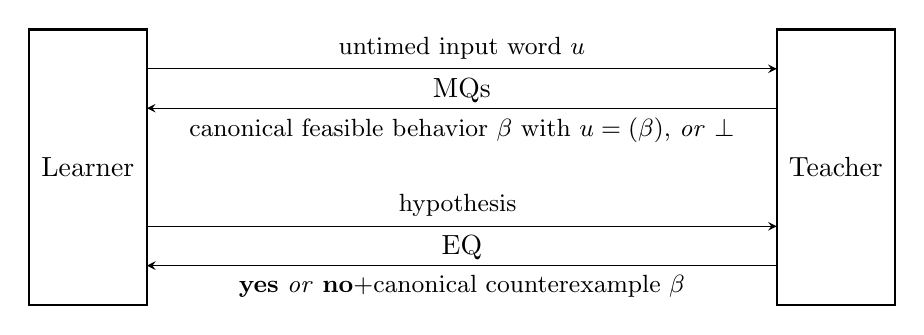
\begin{tikzpicture}[>=stealth]
            \draw [thick] (0,0) rectangle (1.5,3.5) node[midway] {Learner};
            \draw [thick] (9.5,0) rectangle (11,3.5) node[midway] {Teacher};
            \draw [->] (1.5,3) -- (9.5,3) node[midway,below] {MQs};
            \draw (1.5,3) -- (9.5,3) node[midway,above] {\small untimed input word $u$};
            \draw [<-] (1.5,2.5) -- (9.5,2.5) node[midway,below] {\small canonical feasible behavior $\beta$ with $u=\untimedinputword(\beta)$, \emph{or} $\perp$};
            \draw [->] (1.5,1) -- (9.5,1) node[midway,below] {EQ};
            \draw (1.5,1) -- (9.5,1) node[midway,above] {\small hypothesis $\CH$};
            \draw [<-] (1.5,0.5) -- (9.5,0.5) node[midway,below] {\small {\bf yes} \emph{or} {\bf no}+canonical counterexample $\beta$};
        \end{tikzpicture}
\end{center}    
\caption{Untimed MAT framework}
\label{fig:untimed MAT}
\end{figure}
\fi

In our first learning setup, 
\iflong
illustrated in Figure~\ref{fig:untimed MAT},
\fi
the teacher knows an MMT $\M$.
The learner initially knows the set of inputs $I$, and may pose two types of queries.
With a \emph{membership query}, the learner asks for the response to an untimed input word $u$ over $I$.
If $\M$ has a feasible untimed behavior $\beta$ with $\untimedinputword(\can{\beta}) = u$ then the teacher answers
$\can{\beta}$. Otherwise, the answer is $\perp$ (``undefined'').
With an \emph{equivalence query}, the learner asks if a hypothesis $\CH$ with inputs $I$ is correct.
Upon receiving $\CH$, the teacher answers \emph{yes} if $\CH \approx_{\mathit{untimed}} \M$.
Otherwise it answers \emph{no} and supplies a counterexample, a canonical untimed behavior $\beta$ that
is isomorphic to a feasible behavior of $\M$ but not to a feasible behavior of $\CH$.

\subsection{A timed MAT framework for learning MMTs}
In our second learning setup, the teacher also knows an MMT $\M$.
Initially, the timed learner knows the set $I$ of input of $\M$.
The task of the timed learner is to learn $\M$ through three types of queries: membership queries, equivalence queries,
and lookahead queries.

\paragraph{Membership queries.}
A \emph{timed input word} is a sequence
$u = d_1 ~ i_1 \cdots d_k ~ i_k ~ d_{k+1}$, where $d_j \in \delays$ and $i_j \in I$, for all $1 \leq j \leq k$,
and $d_{k+1} \in \realsplus$.
A timed input word describes an experiment that may be carried out on an MMT. We provide a series of inputs at specific times, and record all the outputs that occur in response to these inputs up to and including the finishing time of the experiment, that is $\sum_{j=1}^{k+1} d_j$.
A timed input word is \emph{transparent} if the fractional part of the absolute times of occurrence of
all the inputs are different.
Let $w$ be a timed word.
We associate a unique timed input word $\timedinputword(w)$ to $w$ by 
removing all the outputs events, 
removing all occurrences of $\mathit{to}$, 
replacing consecutive numbers by their sum, 
and possibly placing $0$ at the end of the sequence.
Thus, for instance,
$\timedinputword (3 ~ i_1 ~ o_1 ~ 1.1 ~ i_2 ~ o_2 ~ 2 ~ \mathit{to} ~ o_3 ~ 2.1 ~ i_4 ~ o_4) = 
3 ~ i_1 ~ 1.1 ~ i_2 ~ 4.1 ~ i_4 ~ 0$.

\iflong
Note that the first input occurs at time $3$, the second at time $4.1$, and the third at time $8.2$.
Thus the fractional part of the times of the inputs are different. In fact, $w$ is transparent iff $\timedinputword(w)$ is transparent.
\fi
%
If $u$ and $u'$ are timed input words, then we write $u \propto u'$ if $u$ and $u'$ are equal, except that the final delay of $u$ is less or equal than the final delay of $u'$. Observe that,
for any transparent timed input word $u$ over $I$, 
there exists a unique maximal timed word $w$ of $\M$ such that $\timedinputword(w) \propto u$.
With a \emph{membership query}, the learner asks what the output is in response to a transparent timed input word $u$ over $I$. 
The teacher answers with the unique maximal timed word $w$ of $\M$ such that $\timedinputword(w) \propto u$.

\paragraph{Equivalence queries.}
With an \emph{equivalence query}, the learner asks if a hypothesized MMT $\CH$ is correct, that is, 
whether $\CH \approx_{\mathit{timed}} \M$.
The teacher answers \emph{yes} if this is the case. Otherwise she answers \emph{no} and supplies a
\emph{counterexample}: a transparent timed word $w$ of $\M$ that is not a timed word of $\CH$.
\iflong
(By Lemma~\ref{not timed} 
\else
(We claim that
\fi
such a timed word always exists.)

\paragraph{Lookahead queries.}
A key question that a learner needs to answer is which timers are active after some untimed input word $u$.
Since we assume that there are no ghost variables, a timer that is active after $u$ can expire eventually,
following some further inputs.
In general, however, it may be very difficult to find an input sequence that demonstrates that a timer is active: we may have combination lock scenarios
in which a timer only expires after some very specific, long sequence of inputs.
The search for such a sequence may require an exponential number of membership queries.
However, if when we look at the actual use of timers in protocols, combination lock scenarios just do not occur:
timeouts are not triggered by the occurrence of complicated sequences of inputs, 
but rather by the \emph{absence} of certain inputs.
Simply waiting and providing no inputs at all is usually enough to demonstrate that some timer has been set.
We encapsulate the search for a proof that a timer is active into a \emph{lookahead oracle}:
by posing a \emph{lookahead query}, a timed learner asks if, for some untimed input sequence $u = i_1 \cdots i_k$ and some
index $j \leq k$, timer $x_j$ is active after $u$ in $\M$.
The teacher/oracle answers \emph{yes} if this is the case, and \emph{no} otherwise.
In the case the answer is \emph{yes} and $j=k$ the teacher gives the value to which the timer has just been set.

\subsection{A MAT framework for learning Mealy machines}
We will present an algorithm for an untimed learner, by using existing algorithms for learning Mealy machines as a basis.

A \emph{Mealy machine (MM)} is a tuple $\A = (I, O, Q, q_0, \delta, \lambda)$, where
$I$ is a finite set of inputs,
$O$ is a finite set of outputs,
$Q$ is a finite set of states,
$q_0 \in Q$ is the initial state,
$\delta: Q \times I \rightarrow Q$ is a transition function, and
$\lambda: Q \times I \rightarrow O$ is an output function.
%
Output function $\lambda$ is extended to sequences of inputs by defining,
for all $q \in Q$, $i \in I$ and $\sigma \in I^{\ast}$,
%\begin{eqnarray*}
%\delta(q, \epsilon) = q &,~~~ & \delta(q, i \sigma) = \delta(\delta(q,i), \sigma),\\
$\lambda(q, \epsilon) = \epsilon$ and $\lambda(q, i \sigma) = \lambda(q, i) \lambda(\delta(q, i), \sigma)$.
%\end{eqnarray*}
%
The behavior of Mealy machine $\A$ is defined by function $A_\A : I^{\ast} \rightarrow O^{\ast}$ with
$A_\A(\sigma) = \lambda (q^0, \sigma)$, for  $\sigma \in I^{\ast}$.
Mealy machines $\A$ and $\B$ are \emph{equivalent}, denoted $\A \approx \B$, iff $A_{\A} = A_{\B}$.
Sequence $\sigma \in I^{\ast}$ \emph{distinguishes}
$\M$ and $\N$ iff $A_{\M}(\sigma) \neq A_{\N}(\sigma)$.

In our third learning setup, the teacher knows a Mealy machine $\M$. 
The learner initially knows the inputs $I$ of $\M$ and may ask two types of queries.
With a \emph{membership query}, the learner asks for the response to an input sequence $\sigma \in I^{\ast}$.
The teacher answers with output sequence $A_{\M}(\sigma)$.
With an \emph{equivalence query}, the learner asks if a hypothesized minimal Mealy machine $\CH$ with
inputs $I$ is correct, that is, whether $\CH$ and $\M$ are equivalent.
The teacher answers \emph{yes} if this is the case. Otherwise she answers \emph{no} and supplies a
\emph{counterexample} $\sigma \in I^{\ast}$ that distinguishes $\CH$ and $\M$.

The $L^{\ast}$ algorithm of Angluin \cite{Ang87} is able to learn Mealy machine $\M$ by asking a
number of membership and equivalence queries that polynomial in the size of the corresponding canonical Mealy machine.
Efficient implementations of $L^{\ast}$ and other algorithms for learning Mealy machines are available,
for instance in the tool \learnlib\ \cite{Nie03,RSBM09,MertenSHM11}.

\subsection{A Myhill Nerode Theorem for MMTs}

\begin{definition}
Let $S$ be a set of feasible untimed behaviors in canonical form over $I$ and $O$. Then $S$ is
\emph{prefix closed} if $\beta \beta' \in S \Rightarrow \beta \in S$,
\emph{behavior deterministic} if
$\beta \xrightarrow{i/o_1, \rho_1} X_1 \in S \wedge \beta \xrightarrow{i/o_2, \rho_2} X_2 \in S \Rightarrow o_1 = o_2 \wedge \rho_1 = \rho_2 \wedge X_1 = X_2$,
\emph{input complete} if
$\beta \in S \wedge i \in I \Rightarrow \exists o, \rho, Y : \beta \xrightarrow{i/o, \rho} Y \in S$,
and
\emph{timeout complete} if
$\beta \in S \wedge x \mbox{ expirable after } \beta \Rightarrow
\exists o, \rho, Y: \beta \xrightarrow{\toevent{x}/o, \rho} Y \in S$.

Suppose $\beta$ and $\beta'$ are behaviors in $S$ with $\Last{\beta} = X$ and $\Last{\beta'} = X'$.
Then $\beta$ and $\beta'$ are \emph{equivalent}, written $\beta \equiv_S \beta'$, iff there exists a bijection
$f_0 : X \to X'$ such that for any untimed behavior $\gamma$:
(a) if $\beta \cdot \gamma \in S$ then there exists an isomorphism $f$ that extends $f_0$ such that $\beta' \cdot f(\gamma) \in S$, and conversely,
(b) if $\beta' \cdot \gamma \in S$ then there exists an isomorphism $f$ that extends $f_0^{-1}$ such that $\beta \cdot f(\gamma) \in S$.
We write $[\beta]$ to denote the equivalence class of $\beta$ with respect to $\equiv_S$.
\end{definition}

\begin{theorem}
\label{Myhill Nerode}
Let $S$ be a set of feasible untimed behaviors in canonical form over finite sets of inputs $I$ and outputs $O$.
Then there exists an MMT with feasible untimed behaviors $T$ such that $S = \can{T}$ iff 
$S$ is nonempty, all untimed behaviors in $S$
start with the empty set of timers, $S$ is prefix closed, 
there is a bound on the number of timers that can be active simultaneously 
($\exists n \in \nat ~ \forall \beta \in S : \mid \Last{\beta} \mid \leq n$),
$S$ is behavior deterministic, input complete, timeout complete,
and $\equiv_S$ has only finitely many equivalence classes (finite index).
\end{theorem}
\iflong
\begin{proof} (Needs work)

``$\Rightarrow$'' Let $\M$ be an MMT, let $T$ be its set of feasible untimed behaviors, and let $S = \can{T}$.
Then it is immediate from the definitions that $T$ is nonempty, all untimed behaviors in $S$
start with the empty set of timers, 
$S$ is prefix closed, 
there is a bound on the number of timers that can be active simultaneously,
$S$ is behavior deterministic, input complete, and timeout complete.
Suppose that $\beta, \beta' \in S$.
Then there exist (unique) $\beta_1, \beta'_1 \in T$ with
$\can{\beta_1}=\beta$ and $\can{\beta'_1}=\beta'$.
Suppose $\beta_1$ and $\beta'_1$ lead to the same state $q$ and moreover $\Post_{\beta_1} = \Post_{\beta'_1}$.
Since $\beta$ and $\beta_1$ are isomorphic, and $\beta'$ and $\beta'_1$ are isomorphic,
there exists a bijection $f_0 : X \to X'$ such that $f_0(\Post_{\beta}) = \Post_{\beta'}$.
Suppose that, for some untimed behavior $\gamma$, $\beta \gamma \in S$.
Then there exists an untimed behavior $\gamma_1$ such that $\beta_1 \gamma_1 \in T$ and $\can{\beta_1 \gamma_1} = \beta \gamma$.
By Lemma~\ref{lemma: feasibility concatenation},
$\beta'_1 \cdot \gamma_1 \in T$.
This implies $\beta' f(\gamma) \in S$ (elaborate this).
Since $\M$ only has finitely many states and by Lemma~\ref{lemma finitely many zones} the set
$\{ \Post_{\beta} \mid \beta \mbox{ is a feasible untimed behavior of } \M \}$ is finite, this means that
$\equiv_S$ has finite index.

``$\Leftarrow$'' Suppose $S$ is nonempty, etc.
Let $n$ be a bound on the number of timers that are active in a behavior in $S$ at any point.
We can construct a function that maps each untimed behavior $\beta \in S$
to an isomorphic behavior $\uncan{\beta}$ in such a way that only timers $\{ x_1 ,\ldots, x_n \}$ occur 
in all the behaviors in the range of $\mathit{uncan}$.
For instance, if a transition occurs in a state and this transition
starts a new timer, then $\mathit{uncan}$ may compute the smallest index $j$
such that $x_j$ is not unaffected by this transition, and then choose $x_j$ as the name of the new timer.
Let MMT $\M = (I, O \cup \{ \perp \}, Q, q_0, \vars, \delta, \lambda, \remap)$ be defined as follows:
\begin{itemize}
\item
$\perp$ is a special, fresh output event.
\item
$Q = \{ ( [\beta], \Post_{\uncan{\beta}}) \mid \beta \in S \}$.
\item
$q_0 = ([\emptyset], Z_0)$. (Note that $\emptyset \in S$ since $S$ is nonempty, prefix closed, and all untimed behaviors in $S$ start
with the empty set of timers; $Z_0$ is the unique zone for the empty set of variables.)
\item
$\varsof{([\beta], Z)} = \domof{Z}$.
\item
(rest needs doing). Let $\beta \in S$ and $i \in I$. Then, since $S$ is both input complete and behavior deterministic, there exist unique
$o$, $\rho$ and $Y$ such that $\beta' = \beta \xrightarrow{i/o, \rho} Y \in S$.
We define $\delta([\beta],i) = [\beta']$, $\lambda([\beta],i) = o$, and $\remap([\beta],i) = \rho$.
\item
Assume $\beta \in S$ and $x\in \Last{\beta}$ expirable after $\beta$. 
Then, since $S$ is both timeout complete and behavior deterministic, there exist unique
$o$, $\rho$ and $Y$ such that $\beta' = \beta \xrightarrow{\toevent{x}/o, \rho} Y \in S$.
We define $\delta([\beta],\toevent{x}) = [\beta']$, $\lambda([\beta],\toevent{x}) = o$, and $\remap([\beta],\toevent{x}) = \rho$.
\item
Assume $\beta \in S$ and $x \in \Last{\beta}$ not expirable after $\beta$.
We define $\delta([\beta],\toevent{x}) = [\beta]$, $\lambda([\beta],\toevent{x}) = \perp$, and $\remap([\beta],\toevent{x}) = \rho_0$, where $\domof{\rho_0} = \emptyset$.
\end{itemize}
It is routine to verify that $\M$ is a well-defined MMT whose set of feasible untimed behaviors equals $S$.
\end{proof}
\fi


\subsection{Constructing an untimed MMT learner using a MM learner}
The number of timers that may occur in canonical untimed behaviors grows unboundedly with the length of these behavior,
since timers are never reused in canonical behaviors.
Let $S$ be the set of canonical versions of the feasible untimed behaviors of an MMT $\M$.
Then there is a fixed upper bound on the number of timers that are active in a behavior in $S$ at any point,
since $\M$ only has a finite number of timers that it may use.
This means that we can effectively construct a function that maps each untimed behavior $\beta \in S$
to an isomorphic behavior $\uncan{\beta}$ in such a way that only finitely many
different timers occur in all the behaviors in the range of $\mathit{uncan}$.
For instance, if a transition occurs in a state in which the set of active timers is $Y$, and this transition
starts a new timer, then $\mathit{uncan}$ may compute the smallest index $j$
such that $x_j \not\in Y$, and then choose $x_j$ as the name of the new timer.
Note that that the timers that occur in $\uncan{S}$ may be different from the timers used by $\M$.

Our algorithm for an untimed learner is based on the following result, which is variant of the famous 
Myhill-Nerode theorem for MMTs.

\begin{definition}
\label{def:nerode}
Let $S$ be a set of feasible untimed behaviors over $I$. Then $S$ is
\emph{prefix closed} if $\beta \beta' \in S \Rightarrow \beta \in S$,
\emph{behavior deterministic} if
$\beta \xrightarrow{i/o_1, \rho_1} X_1 \in S \wedge \beta \xrightarrow{i/o_2, \rho_2} X_2 \in S \Rightarrow o_1 = o_2 \wedge \rho_1 = \rho_2 \wedge X_1 = X_2$,
\emph{input complete} if
$\beta \in S \wedge i \in I \Rightarrow \exists o, \rho, Y : \beta \xrightarrow{i/o, \rho} Y \in S$,
and
\emph{timeout complete} if
$\beta \in S \wedge x \mbox{ expirable after } \beta \Rightarrow
\exists o, \rho, Y: \beta \xrightarrow{\toevent{x}/o, \rho} Y \in S$.
Behaviors $\beta, \beta' \in S$ are \emph{equivalent} for $S$, notation $\beta \equiv_S \beta'$, iff 
for any untimed behavior
$\gamma$, $\beta \cdot \gamma \in S \Leftrightarrow \beta' \cdot \gamma \in S$.
We write $[\beta]$ to denote the equivalence class of $\beta$ with respect to $\equiv_S$.
\end{definition}

\begin{theorem}
\label{Nerode theorem}
Let $S$ be a set of feasible untimed behaviors over finite sets of inputs $I$ and outputs $O$.
Then $S$ is the set of feasible untimed behaviors of an MMT $\M$ iff $S$ is nonempty, all untimed behaviors in $S$
start with the empty set of timers, the set of timers that occur in $S$ is finite,
$S$ is prefix closed, behavior deterministic, input complete, timeout complete,
and $\equiv_S$ has only finitely many equivalence classes (finite index).
\end{theorem}
\iflong
\begin{proof}

``$\Rightarrow$'' Let $\M$ be an MMT and let $S$ be the set of its feasible untimed behaviors.
Then it is immediate from the definitions that $S$ is nonempty, all untimed behaviors in $S$
start with the empty set of timers, the set if timers that occurs in $S$ is finite,
$S$ is prefix closed, behavior deterministic, input complete, and timeout complete.
Suppose that feasible untimed behaviors $\beta$ and $\beta'$ lead to the same state $q$ and moreover $\Post_{\beta} = \Post_{\beta'}$.
Then, 
by Lemma~\ref{lemma: feasibility concatenation},
for any untimed behavior $\gamma$, $\beta \cdot \gamma \in S \Leftrightarrow \beta' \cdot \gamma \in S$, and thus
$\beta \equiv_S \beta'$.
Since $\M$ only has finitely many states and by Lemma~\ref{lemma finitely many zones} the set
$\{ \Post_{\beta} \mid \beta \mbox{ is a feasible untimed behavior of } \M \}$ is finite, this means that
$\equiv_S$ has finite index.

``$\Leftarrow$'' Suppose $S$ is nonempty, etc.
Let MMT $\M = (I, O \cup \{ \perp \}, Q, q_0, \vars, \delta, \lambda, \remap)$ be defined as follows:
\begin{itemize}
\item
$\perp$ is a special, fresh output event.
\item
$Q$ is the set of equivalence classes of $\equiv_S$.
\item
$q_0 = [\emptyset]$. (Note that $\emptyset \in S$ since $S$ is nonempty, prefix closed, and all untimed behaviors in $S$ start
with the empty set of timers.)
\item
$\varsof{[\beta]} = \Last{\beta}$.
\item
Let $\beta \in S$ and $i \in I$. Then, since $S$ is both input complete and behavior deterministic, there exist unique
$o$, $\rho$ and $Y$ such that $\beta' = \beta \xrightarrow{i/o, \rho} Y \in S$.
We define $\delta([\beta],i) = [\beta']$, $\lambda([\beta],i) = o$, and $\remap([\beta],i) = \rho$.
\item
Assume $\beta \in S$ and $x\in \Last{\beta}$ expirable after $\beta$. 
Then, since $S$ is both timeout complete and behavior deterministic, there exist unique
$o$, $\rho$ and $Y$ such that $\beta' = \beta \xrightarrow{\toevent{x}/o, \rho} Y \in S$.
We define $\delta([\beta],\toevent{x}) = [\beta']$, $\lambda([\beta],\toevent{x}) = o$, and $\remap([\beta],\toevent{x}) = \rho$.
\item
Assume $\beta \in S$ and $x \in \Last{\beta}$ not expirable after $\beta$.
We define $\delta([\beta],\toevent{x}) = [\beta]$, $\lambda([\beta],\toevent{x}) = \perp$, and $\remap([\beta],\toevent{x}) = \rho_0$, where $\domof{\rho_0} = \emptyset$.
\end{itemize}
It is routine to verify that $\M$ is a well-defined MMT whose set of feasible untimed behaviors equals $S$.
\end{proof}
\fi

The canonical MMT $\M$ constructed in the proof of Theorem~\ref{Nerode theorem} has a special property: an untimed
behavior of $\M$ is feasible iff it does not contain
\iflong
the
\else
a
\fi
special output event $\perp$. Call an MMT that satisfies this property
\emph{transparent}. 
We say that a timer $x$ \emph{may expire} in a state $q$ if $q$ has an outgoing $\toevent{x}$ transition with
an output different from $\perp$.
In a transparent MMT, a timer may expire after an untimed behavior $\beta$ iff it may expire in the
unique state of $\M$ that is reached by $\beta$.
%
Note that, for any MMT $\N$ there exists an equivalent transparent MMT $\M$, since
from the set $S$ of feasible untimed behaviors of $\N$ we may construct an equivalent transparent MMT using the construction
of Theorem~\ref{Nerode theorem}.
Our learning algorithm requires a number of queries that is polynomial in the size of the minimal transparent MMT that is equivalent to the given MMT.

Our algorithm for an MMT learner works as follows.
Let $S$ be the set of canonical versions of feasible untimed behaviors of $\M$.
The MMT learner guesses an overapproximation $Y$ of the set of timers that occur in $\uncan{S}$.
(If this guess turns out to be wrong the learner extends $Y$ and restarts the learning process.)
Next it starts a MM learner with a set of input actions $I' = I \cup \{ \toevent{x} \mid x \in Y \}$.
Since Mealy machines are input enabled, membership queries posed by the MM learner will in general contain
inputs $\toevent{x}$ which are either \emph{illegal}, when timer $x$ is not currently active, or \emph{infeasible},
meaning that timer $x$ cannot expire in the current state.
Inputs which are neither illegal or infeasible are called \emph{good}.
Suppose that the MM learner poses a membership query $\sigma$.
Step by step, by computing the untimed input words that correspond to prefixes with good inputs in $\sigma$, 
and by posing corresponding membership queries,
the MMT learner figures out which inputs are illegal or infeasible, and what is the output and update for each good input.
%induced by the valid inputs up to $i_j$.
%The initial untimed behavior $\beta_0 = \emptyset$.
%Suppose that the learner has figured out which inputs in $u_j = i_1 \cdots i_{j-1}$ are bad and which untimed behavior
%$\beta_j$ is induced by the good inputs in $u_j$. If $i_j = \toevent{x}$ with $x \not\in X_{j-1}$ then input $i_j$ is illegal.
%Otherwise the MMT learner submits a membership query $\untimedinputword(\can{\beta_j}) ~ i_j$.
%If the response is $\perp$ then input $i_j$ is infeasible.
%Otherwise the response is $\can{\beta}$
%as 
Based on this an anwer for query $\sigma$ can be computed:
in response to an illegal input the MMT learner returns $\ast$, 
in response to an infeasible input it returns $\perp$,
and in response to a good input it returns the corresponding output/update pair obtained via the MMT membership queries.

If the MM learner poses an equivalence query, this will be a minimal Mealy machine $\CH$ in which the illegal
inputs correspond to self-loops with output $\ast$. Based on the $\ast$-loops we can
determine the functions $\vars$, that is, the set of active timers in each state. By removing the $\ast$-loops we
obtain an MMT $\CH'$, which the MMT learner forwards as an equivalence query.
If the hypothesis is incorrect and the MMT learner receives a counterexample $\beta$,
it forwards counterexample $\untimedinputword(\uncan{\beta})$ to the MM learner.

%Let $\M = (I, O, Q, q_0, \vars, \delta, \lambda, \remap)$ be a transparent MMT with $\perp \in O$.
%Let $Y = \bigcup_{q \in Q} \varsof{q}$ be the set of timers that appear in $\M$.
%We associate to $\M$ a Mealy machine $\Mealy(\M) = (I', O', Q, q_0, \delta', \lambda')$ where
%\begin{itemize}
%\item
%$I' = I \cup \{ \toevent{x} \mid x \in Y \}$
%\item
%$O' = O \times (X \hookrightarrow \natplus)$
%\item
%$\delta'(q,i) = \left\{ \begin{array}{ll}
%\delta(q,i) & \mbox{if } i \in I \mbox{ or } \exists x \in \varsof{q} : i = \toevent{x} \mbox{ and } \lambda(q,i) \neq \perp\\
%q & \mbox{otherwise}
%\end{array} \right.$
%\item
%$\lambda'(q,i) = \left\{ \begin{array}{ll}
%(\lambda(q,i), \rho(q,i), \varsof{q}) & \mbox{if } i \in I \mbox{ or } \exists x \in \varsof{q} : i = \toevent{x} \mbox{ and } \lambda(q,i) \neq \perp\\
%(\perp,\emptyset) & \exists x \in \varsof{q} : i = \toevent{x} \mbox{ and } \lambda(q,i) = \perp\\
%(\ast,\emptyset) & \mbox{otherwise}
%\end{array} \right.$
%\end{itemize}
%
%\begin{theorem}
%\label{untimedequivalentmealy}
%Let $\M$ and $\N$ be transparent MMTs.
%Then $\M \approx_{\mathit{untimed}} \N$
%iff
%$\Mealy(\M) \approx \Mealy(\N)$.
%\end{theorem}

\subsection{Constructing an untimed MMT teacher using a timed teacher}
In this subsection, we show how we may construct a teacher for the untimed setting by using a teacher for the timed setting.

Suppose the untimed teacher receives a membership query, consisting of an untimed input word
$u = i_1 \cdots i_k$.
Inductively, we construct a response for $u$, that is a canonical untimed behavior $\beta$ that is
isomorphic to a feasible untimed behavior of $\M$ with $\untimedinputword(\beta) = u$,
or $\perp$ if such a word does not exist.
If $k=0$, then we take $\beta = \emptyset$.
For the induction step, suppose that $k>0$.
If the response for $i_1 \cdots i_{k-1}$ is $\perp$, then the answer for $u$ is also $\perp$.
Otherwise, let $\beta$ be the response for $i_1 \cdots i_{k-1}$.
If $i_k = \toevent{x}$ for some timer $x$ that is not expirable after $\beta$ then there exists no feasible behavior
with untimed input word $u$. In this case, the untimed teacher may return the answer $\perp$.
Otherwise, there exists a feasible behavior that extends $\beta$ with input $i_k$. We compute
a corresponding transparent timed behavior, extract a timed input word from it and pose this as a query to the timed learner.
Since the resulting timed word is transparent, it has a unique causality map, so we know
which timeouts and outputs occur.
Using a series of lookahead queries, we can determine which timers are active at each point during the run,
and which timers have been set that have not yet timed out.
Based on this, the untimed MMT teacher may answer the membership query.

Once we have implemented membership queries, implementing equivalence queries is easy.
Suppose that the untimed teacher receives an equivalence query $\CH$.
Then we just forward this query to the timed teacher.
If the timed teacher answers \emph{yes} then $\CH \approx_{\mathit{timed}} \M$.
In this case, by Theorem~\ref{timedimpliesuntimed}, $\CH \approx_{\mathit{untimed}} \M$,
and thus the untimed teacher can also return a result \emph{yes}.
If the timed teacher answers \emph{no} and returns a counterexample $w$,
then $w$ is a transparent timed word of $\M$ but not of $\CH$.
In this case, by Theorem~\ref{untimedimpliestimed}, we may conclude that
$\CH \not\approx_{\mathit{untimed}} \M$, and thus the untimed teacher can also return a result \emph{no}.
Since $w$ is a transparent timed word of $\M$, it 
\iflong
follows by Lemma~\ref{lemma unique causality map} that $w$ 
\fi
has a unique causality map $c$.
This allows us to transform $w$ into an untimed input sequence $u$: 
we remove all the delays and output events, and if the $j$-th
input in $w$ equals $\mathit{to}$, we replace it by $\toevent{x_{c(j)}}$.
The untimed teacher performs an untimed membership query for $u$, and returns the resulting 
untimed behavior $\beta$ as counterexample.






